\documentclass{article}
\usepackage[utf8]{inputenc}
\usepackage[table]{xcolor}
\usepackage{graphicx}
\usepackage[T1]{fontenc}
\usepackage{imakeidx}
\usepackage{imakeidx}
\usepackage{tabularx}
\usepackage{booktabs}
\usepackage{outlines}
\usepackage{forloop}
\usepackage{pgfgantt}
\usepackage{xcolor,colortbl}
\makeindex[name=Alphabetical,title={Alphabetical Index},columns=1]
\makeindex[name=Functions,title={Index of Functions},columns=1]

\newcounter{loopcntr}
\newcommand{\rpt}[2][1]{%
  \forloop{loopcntr}{0}{\value{loopcntr}<#1}{#2}%
}
\newcommand{\on}[1][1]{
  \forloop{loopcntr}{0}{\value{loopcntr}<#1}{&\cellcolor{gray}}
}
\newcommand{\off}[1][1]{
  \forloop{loopcntr}{0}{\value{loopcntr}<#1}{&}
}


\title{Requirements rapport - Softwareteknologi} % Sets article title
\author{Artin Ghalamkary - (AU677595) \and Karsten Bak Malle - (AU644054) \and Nikita Svanholm Alsøer - (AU639436) \and Phillip Ravn Boe Jensen - (AU681033)}% Sets authors name
\date{01-10-2021}

\begin{document}

\maketitle
\section*{Preface} \index[Alphabetical]{Preface}
The requirements rapport document include some documentation that describe our mail clients behavior and some of its features. Such documentation consists of data flow models and a system architecture or a definition of functional and nonfunctional requirements. This specific requirements rapport may not contain every detail or capture every element of our mail clients behavior and feature, because the client is in early stages of development, and the customers needs may change during the process of creating the mail client. It is expected that the requirements will change in the future, presumably with more in-depth description and with additional functionalities. \\


\section*{Introduction} \index[Alphabetical]{Introduction}
The purpose of our email client is to provide a secure service that allows the customer to communicate to others through emails. The email client will have various functions some being the essentials such as displaying, sending and deleting mails. Other functions could be the likes of blacklisting emails or attaching files/pictures to the mail. The email client will work together with a server that fetched and send emails to other recipients. 

\newpage
\section*{Glossary} \index[Alphabetical]{Glossary}

\begin{enumerate}
    \item \textbf{Database:}\index[Alphabetical]{Database} A Database is an organized collection of information/data, that is stored electronically in a computer system.
    \item \textbf{Agile process:}\index[Alphabetical]{Agile process} The Agile process is a way to manage a project by breaking it up into several phases. It involves constant collaboration with the customer and continuous improvement at every stage. Once the work begins, teams cycle through a process of planning, executing, and evaluating.
    \item \textbf{Plan-driven development process:}\index[Alphabetical]{Plan-driven development process} The Plan-driven development process attempts to plan and anticipate all the features the customer might want in the product and the way to build these features, before creating any software.  
    \item \textbf{System architecture:}\index[Alphabetical]{System architecture} The System architecture gives us a visual representation of the concepts behind the structure and behavior of the system, and it shows the relationship and interaction between the features of the system.
    \item \textbf{System model}:\index[Alphabetical]{System model} The Systems Model is a abstract model of the system, representing the system using graphical notation, typically UML(Unified Modeling Language). 
\end{enumerate}

\newpage

\section*{User requirements definition}\index[Alphabetical]{User requirements definition}
\definecolor{cornflowerblue}{rgb}{0.39, 0.58, 0.93}

\vspace{5 mm}

\centerline{
\begin{tabular}{| c |}
 \hline
 User requirements\\
 \hline 
 \rowcolor{cornflowerblue}
 1. Mail client should be able to display\index[Functions]{Display}, send\index[Functions]{Send}, and receive\index[Functions]{Receive} emails as well as let the user be able & \rowcolor{cornflowerblue} to reply\index[Functions]{Reply} and forward\index[Functions]{Forward} the emails received through the selected server. \\
 \hline
 \rowcolor{cornflowerblue}
 2. Mail client should provide the user the opportunity to login\index[Functions]{Login} to their personal email\\
 \hline
 \rowcolor{cornflowerblue}
 3. The user should be able to blacklist\index[Functions]{Blacklist} any email\\
 \hline
 \rowcolor{cornflowerblue}
 4. The user should be able to login to multiple emails\index[Functions]{Online - multiple emails} at the same time\\
 \hline
 \rowcolor{cornflowerblue}
 5. The user should be able to delete\index[Functions]{Delete} any email\\
 \hline
 \rowcolor{cornflowerblue}
 6. The user should be able to mark emails as read/unread\index[Functions]{Mark - read/unread}\\
 \hline
 \rowcolor{cornflowerblue}
 7. The user should be able attach files and pictures\index[Functions]{Attach files/pictures} to their emails\\
 \hline
 \rowcolor{cornflowerblue}
 8. The user should be able to compose\index[Functions]{Compose} a email\\

\end{tabular}
}

\vspace{5 mm}

\begin{center}
\begin{tabular}{| c |}
 \hline
 Nonfunctional requirements\\
 \hline 
 \rowcolor{cornflowerblue}
 1. Limited database \\
 \hline
 \rowcolor{cornflowerblue}
 2. Interval of email fetching\\
 \hline
 \rowcolor{cornflowerblue}
 3. Mail client will be driven by localhost\\
 \hline
 \rowcolor{cornflowerblue}
 4. Mail client downtime\\
 \hline
 \rowcolor{cornflowerblue}
 5. File attachment size constraint\\
 \hline
\end{tabular}
\end{center}

\newpage

\section*{System architecture}\index[Alphabetical]{System architecture}
\vspace{8 mm}

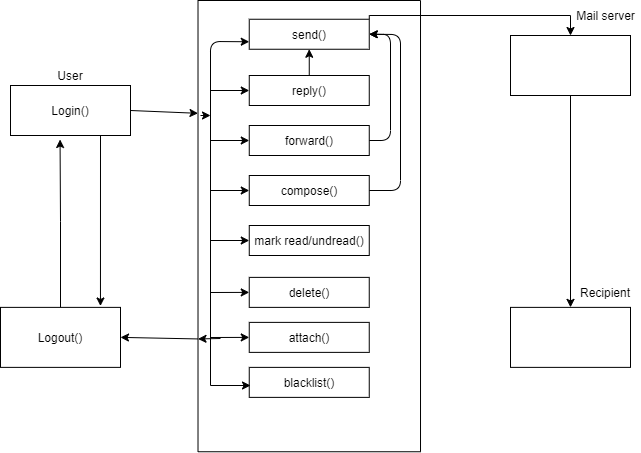
\includegraphics[width=300px, keepaspectratio]{System architecture.drawio.png}\\[1cm]\index[Alphabetical]{System architecture diagram}

\vspace{-15 mm}

\newpage
\section*{System requirements specification}\index[Alphabetical]{System requirements specification}

\begin{enumerate}
    \item \textbf{Attach files/pictures:}\index[Functions]{Attach files/pictures} When sending an email the customer should have the ability to attach a given file or picture alongside the email. It should be noted that the file and picture cannot exceed a fixed size. 
    \item \textbf{Blacklist:}\index[Functions]{Blacklist} The customer should have the ability to register any mail in the blacklist, which function is to separate any emails, which email address has been blacklisted, into another folder. The customer should also have the ability to remove any email address from the blacklist, which will allow future emails from the address back into the main inbox.
    \item \textbf{Compose:}\index[Functions]{Compose} The customer should be able to compose an email, and be allowed to send the mail to a given email address.
    \item \textbf{Delete:}\index[Functions]{Delete} The customer can delete any email, and the deleted email will be moved to the "deleted mail" folder. Within the "deleted mail" folder, the mail will be permanently deleted after 30 days.
    \item \textbf{Display:}\index[Functions]{Display} The server client will visually display the email to the customer. 
    \item \textbf{Forward:}\index[Functions]{Forward} The customer will be able to send a copy of an email they received to a single or several email addresses. 
    \item \textbf{Login:}\index[Functions]{Login} The customer can login with own unique account.
    \item \textbf{Mark - read/unread:}\index[Functions]{Mark - read/unread} The customer will be able to mark emails as read or unread. A email that has already been read can still be marked as unread and the other way around.
    \item \textbf{Online - multiple emails:}\index[Functions]{Online - multiple emails} The customer will be able to login on multiple email accounts at the same time. 
    \item \textbf{Receive:}\index[Functions]{Receive} The customer can receive emails from emails addresses. 
    \item \textbf{Reply:}\index[Functions]{Reply} When receiving an email the customer should have the ability to reply the following email.
    \item \textbf{Send:}\index[Functions]{Send} The customer will be able to send an email to another email address, which will be send using a server.
\end{enumerate}

\section*{System model}\index[Alphabetical]{System model}
\vspace{8 mm}

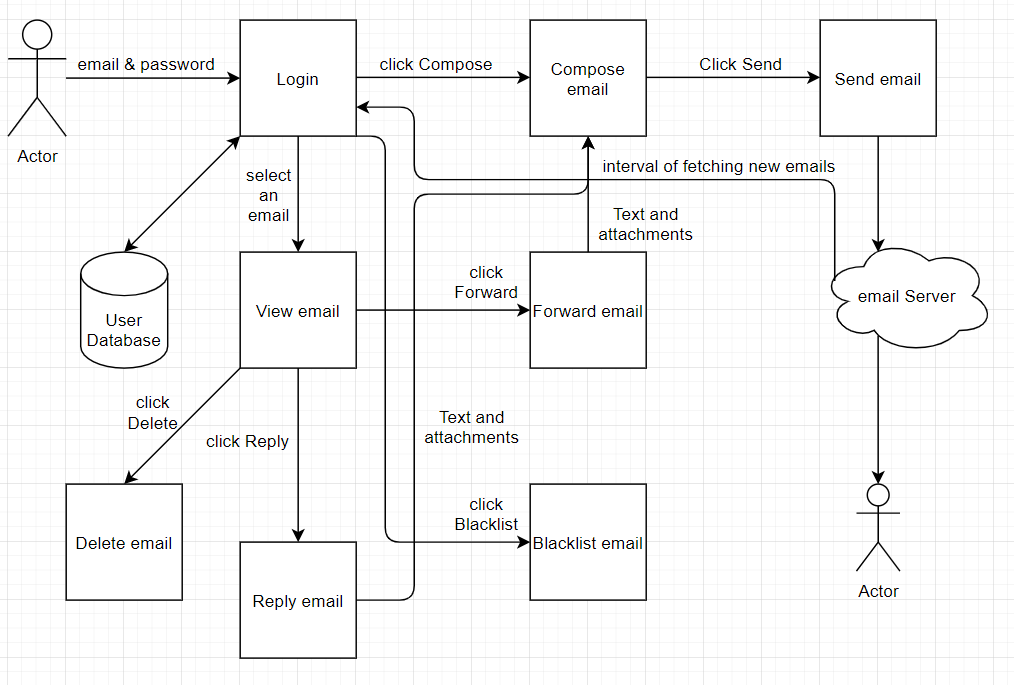
\includegraphics[width=350px, keepaspectratio]{Dataflowchart.png}\\[1cm]\index[Alphabetical]{System model diagram}

\section*{System evolution}\index[Alphabetical]{System evolution}
The thought process behind our system has been to create a symbiosis between the plan driven development, as well as the agile process. To prepare system evolution our focus going forward is to be aware of the implementation of the the agile process, since the system will be required to change, due to  as the user needs change as well. 

\newpage

\section*{Appendices}\index[Alphabetical]{Appendices}
\textbf{Database:} The database will be developed through the usage of the Django framework.
\\
\textbf{Application/Client:} The client will be a build as a web application.

\begin{table}[h]
\centering
    \caption{Hardware requirements} \index[Alphabetical]{Hardware requirements}
    \label{crouch}
    \begin{tabular}{  l  p{3.4cm}  p{3.4cm} }
        \toprule
\textbf{Component}      
& \textbf{Minimum}   
& \textbf{Recommended} \\\midrule
Processor
& 1.9 gigahertz (GHz) x86- or x64-bit dual core processor with SSE2 instruction set        
& 3.3 gigahertz (GHz) or faster 64-bit dual core processor with SSE2 instruction set \\\hline
Memory       
& 2-GB RAM                         
& 4-GB RAM or more  \\\hline
Display       
& Super VGA with a resolution of 1024 x 768 
& Super VGA with a resolution of 1024 x 768 \\
        \bottomrule
    \end{tabular}
\end{table}

\begin{flushleft}
\textbf{Network requirements:}\\ \index[Alphabetical]{Network requirements}

Model-driven apps are designed to work best over networks that have the following elements:
\end{flushleft}
\begin{outline}
    \1 Bandwidth greater than 50 KBps (400 kbps)
    \1 Latency under 150 ms
\end{outline}

\begin{flushleft}
\textbf{Supported web browsers:}\\ \index[Alphabetical]{Supported web browsers}

The web application can run in any of the following web browsers running on the specified operating systems:
\end{flushleft}
\begin{outline}
    \1 Mozilla Firefox (latest publicly-released version) running on Windows 10, Windows 8.1, Windows 8, or Windows 7
    \1 Google Chrome:
        \2 Google Chrome (latest publicly-released version) running on Windows 10, Windows 8.1, Windows 8, Windows 7
        \2 Google Chrome (latest publicly-released version) running on the two latest publicly-release Mac OS versions
    \1 Apple Safari (latest publicly-released version) running on the two latest publicly-release Mac OS versions, or Apple iPad
\end{outline}
\newpage

\section*{Work Plan:}\index[Alphabetical]{Work Plan}

\textbf{Role assignments:}\index[Alphabetical]{Role assignments}
\begin{enumerate}
    \item \textbf{Front-end:} Karsten
    \item \textbf{Middle-end:} Artin \& Nikita
    \item \textbf{Back-end:} Phillip
\end{enumerate}

\vspace{2cm}
\begin{center}
\noindent \begin{tabular}{p{0.251\textwidth}*{12}{|p{0.023\textwidth}}|}
\textbf{}
    & \multicolumn{4}{c|}{October} 
    & \multicolumn{5}{c|}{November} 
    & \multicolumn{3}{c}{December} \\
& \centering{1} & 11 & 15 & 25 & \centering{1} & 15 & 19 & 20 & 30 & \centering{1} & \centering{3} & \multicolumn{1}{c}{10} \\
\hline
Requirements document and work plan & \cellcolor{black} &&&&&&&&&& \\
\hline
\mbox{Send and} \mbox{receive emails} & & \cellcolor{black} &&&&&&&&& \\
\hline
\mbox{Architecture and} \mbox{design document} & && \cellcolor{black} &&&&&&&& \\
\hline
\mbox{User interface} \mbox{layout} & &&& \cellcolor{black} &&&&&&& \\
\hline
Basic requirements \vspace{4mm} & &&&& \cellcolor{black} &&&&&& \\
\hline
\mbox{Functional} \mbox{requirements} & &&&&& \cellcolor{black} &&&&& \\
\hline
Testing \vspace{4mm} & &&&&&& \cellcolor{black} &&&& \\
\hline
Debugging \vspace{4mm} & &&&&&&& \cellcolor{black} &&& \\
\hline
Final testing \vspace{4mm} & &&&&&&&& \cellcolor{black} && \\
\hline
Product draft \vspace{4mm} & &&&&&&&&& \cellcolor{black} & \\
\hline
\mbox{Finalization} \mbox{of product} & &&&&&&&&&& \cellcolor{black}  \\
\hline
Report finalized \vspace{4mm} & &&&&&&&&&&& \cellcolor{black} \\
\hline
\end{tabular}
\end{center}


\printindex[Alphabetical]
\printindex[Functions]





\end{document}

